\chapter{Problem Definition \& Challenges\label{cha:problem-definition}}
This part structures the problem. The problem here is mainly resource allocation and its usage. What are the technical and the theoretical challenges?

\section{Load Balancing Among Fog Nodes}
In a Node-RED context, a service can be seen as a Node-RED \textit{flow} and consists of several \textit{tasks} (functions in a flow), whereas each function could be executed on a different node.
The challenge here is to decide which node should execute which function (see figure \ref{fig:distributed-flow}).
The goal is to meet the service's QoS requirements.
For the MWSN use cases it has to be ensured that a result is available within the defined maximum latency timespan, e.g. within 10ms for condition monitoring for safety.\\

\begin{figure}
    \centering
    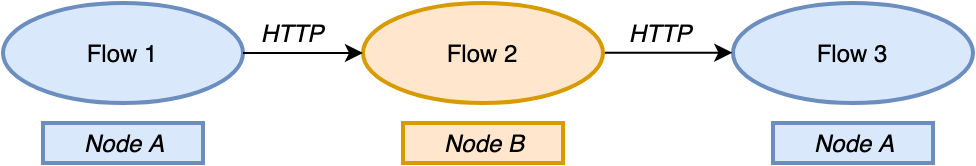
\includegraphics[width=12cm]{architecture-distributed-flow}
    \caption{Distributed flow}
    \label{fig:distributed-flow}
\end{figure}

Fog infrastructure is characterized by different nodes offering various hardware and software resources.
In order to assign tasks to nodes, it must first be checked whether a node is able to execute the task with given QoS requirements.\\

The challenge here is to implement a resource allocation algorithm for the given use cases.


\section{Dynamically Varying Network Conditions}
The network conditions might change at any point in time.
The increased demand for services plays a major role here, but there may also be increased network traffic.
For instance, in the MWSN scenario, the amount of sensors requesting services might increase, which leads to a higher load on the fog nodes hardware until the point of congestion.
To avoid congestion and ensure QoS, tasks of services with a lower priority have to be moved elsewhere to free resources for high priority services.
Apart from that, the network traffic might increase due to other network services which are not part of the fog infrastructure but are using the same link.\\

The challenge here is to adapt to the mentioned changes, for which they must be identified first before the load balancing algorithm is executed to eventually calculate a differentiated, optimized deployment.

\section{Fog Node Failures}
A fog infrastructure is not as reliable as a cloud infrastructure, for instance.
Fog nodes can join or leave the network at any point in time, which leads to a dynamic change in the available resources.
Since fog nodes can be any type of hardware, it is not unlikely that small and relatively cheap devices (e.g. Raspberry Pi) are used.
Thus, it is more likely that they might fail since the hardware components are not of high quality compared to enterprise server hardware.
Furthermore, the environment is neither monitored nor controlled like a cloud server data center, which could lead to node failures (e.g. network connection errors or power supply failures).\\

The challenge here is to adapt to those dynamic changes.
If a node leaves the network, fewer resources are available and therefore another deployment might be the optimum.
Similarly, when a node joins the network, more resources are available, making another deployment ideal.
